\documentclass[]{scrartcl}
\usepackage{graphicx}
\usepackage{geometry}
\geometry{
	a4paper,
	total={170mm,257mm},
	left=20mm,
	top=20mm,
}


%opening
\title{SDD -Hearts Low Level Design}
\author{Brandon Smith, Nieka Gutenberger, Joseph Coppin, Ryan Frazier, Trevor Jewkes}

\begin{document}

\maketitle
\pagebreak
	
	\noindent\makebox[\textwidth{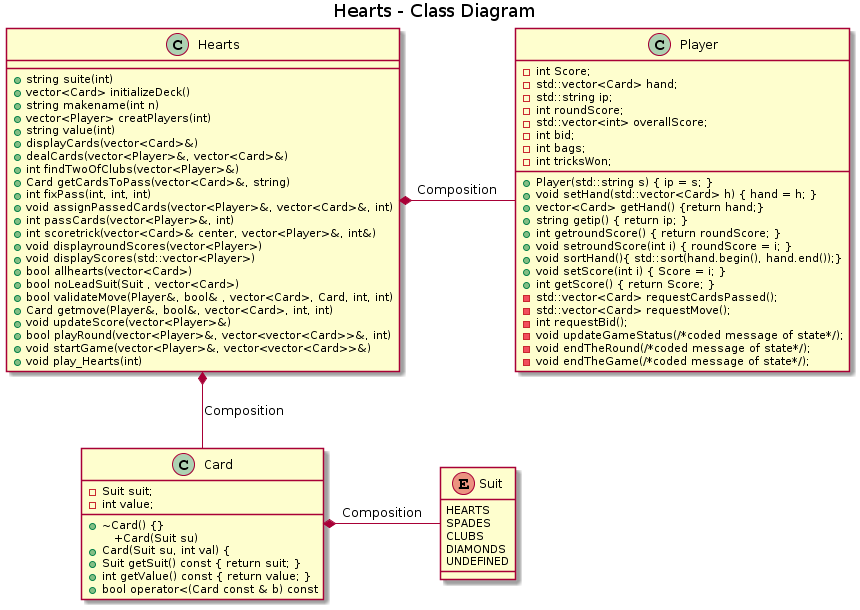
\includegraphics[width=\textwidth]{hearts.png}}]

\section{Hearts Class}

	\begin{itemize}
		\item string suite(int i)
			\begin{itemize}
				\item Converts enum of ints to string of card suit.
			\end{itemize}
		\item vector $\langle$Card$\rangle$ initializeDeck()
			\begin{itemize}
				\item Creates deck of cards taken from card class.
			\end{itemize}
		\item string makename(int n)
			\begin{itemize}
				\item 	Creates a player name.
			\end{itemize}
		\item vector$\langle$Player$\rangle$  creatPlayers(int p)
			\begin{itemize}
				\item Creates a vector of Players to play the game.
			\end{itemize}
		\item void displayCards(vector$\langle$Card$\rangle$ \& hand)
			\begin{itemize}
				\item Displays the deck for screen purposes.
			\end{itemize}
		\item void dealCards(vector$\langle$Player$\rangle$ \& players, vector$\langle$Card$\rangle$ \& Deck)
			\begin{itemize}
				\item Deals cards to players.
			\end{itemize}
		\item int findTwoOfClubs(vector$\langle$Player$\rangle$ \& p)
			\begin{itemize}
				\item Looks through each hand to find the 2 of clubs to find starting player and hand.
			\end{itemize}
		\item Card getCardsToPass(vector$\langle$Card$\rangle$ \& h, string p)
			\begin{itemize}
				\item Gets and stores cards for passing at the beginning of each round.
			\end{itemize}
		\item int fixPass(int r, int p, int c)
			\begin{itemize}
				\item Ensures that cards are passed to the right players depending on the round.
			\end{itemize}
		\item void assignPassedCards(vector$\langle$Player$\rangle$ \& p, vector$\langle$Card$\rangle$ \& h, int r)  
			\begin{itemize}
				\item Takes the passed cards and redistributes based on round.
			\end{itemize}
		\item int passCards(vector$\langle$Player$\rangle$ \& p, int round) 
			\begin{itemize}
				\item Function for passing cards at beginging of round.
			\end{itemize}
		\item int scoretrick(vector$\langle$Card$\rangle$ \& center, vector$\langle$Player$\rangle$ \& players, int\& turn)
			\begin{itemize}
				\item 	Holds the score for the current trick.
			\end{itemize}
		\item void displayroundScores(vector$\langle$Player$\rangle$ p)
			\begin{itemize}
				\item Displays scores for the round.
			\end{itemize}
		\item void displayScores(vector$\langle$Player$\rangle$  p)
			\begin{itemize}
				\item Display scores each turn.
			\end{itemize}
		\item bool allhearts(vector$\langle$Card$\rangle$ h)
			\begin{itemize}
				\item Checks to see if a players hand is all hearts.
			\end{itemize}
		\item string value(int i)
		\item bool noLeadSuit(Suit s, vector$\langle$Card$\rangle$ h)
			\begin{itemize}
				\item Compares hand against the lead suit
			\end{itemize}
		\item bool validateMove(Player\& p, bool\& broken, vector$\langle$Card$\rangle$  Center, Card move, int t, int i)
		\item Card getmove(Player\& p, bool\& b, vector$\langle$Card$\rangle$  c, int t, int i)
		\item void updateScore(vector$\langle$Player$\rangle$ \& p)
			\begin{itemize}
				\item Adds round score to Score.
			\end{itemize}
		\item bool playRound(vector$\langle$Player$\rangle$ \& players, vector$\langle$vector$\langle$Card$\rangle$ $\rangle$\& history, int round)
		\item void startGame(vector$\langle$Player$\rangle$ \& players, vector$\langle$vector$\langle$Card$\rangle$ $\rangle$\& history) 
			\begin{itemize}
				\item  Uses players and calls round until game is over
			\end{itemize}
		\item void play\_Hearts(int num)

	\end{itemize}

\end{document}
